\section{Group Chat}
\label{sec:groupchat}
With the MS5 we extended our program with a group chat feature which enables clients to exchange messages with each other through chatrooms. Additionally, we developed our group chat in such a way that clients can access the DB while being in a chatroom with the help of a chatbot.
 
In the following, the basic functionalities of the group chat are described step by step, subsequently the chat system and its components are examined in depth. Lastly, we discuss how client can access the DB while chatting.

\subsection{Basic Functionalities}
\label{sec:groupchat_functionalities}
To start off, in the same sense as MS4, the External Configuration Service (ECS), where the storage servers are monitored and controlled, is started. Following that a number of servers are created. A client must connect to one of the servers.

\subsubsection{Unique Username}
\label{sec:groupchat_funtionalities_uniqueusername}
After successfully connecting to a key-value server, the client has to either enter a username or use the command "QUIT" to have a username randomly assigned to him. Usernames are implemented as globally unique identifiers for the clients, which prevents different clients from having the same username in different chatrooms. That way, users are guaranteed to know who they are communicating with, as long as their partner is connected to the system.
In order to avoid unnecessary extra connections, the ECS stores a list of users. Whenever a client connects and tries to set its username, the request gets sent through the server to the ECS, which then checks if the username has been already taken by a client connected to any of the servers online. The end user either receives a welcome message with the username displayed if the operation was succesful, or an error message.
 
\subsubsection{Chatrooms}
\label{sec:groupchat_funtionalities_chatcommand}
In order to use to start chatting, the client has to join a chatroom. This is done by typing \texttt{chat} and providing the ID of the chatroom. In case the room does not exist, the user is allowed to create one. The next time a user executes the \texttt{chat} command with the same chatID, he is either granted access to it immediately if it is a public room, or is otherwise first required to enter the password chosen by the person who created the room. The password is hashed on the client side for safety measures and only the hash is required to validate the password attempt.
Each server owns a list containing the active chatrooms that it is responsible for depending on its position on the hash ring. In order for a client to join one of those chatrooms, is that it would first need to connect to that server, similar to the way storing key-value pair works.

\subsubsection{Saved Messages}
\label{sec:groupchat_funtionalities_savedmessages}
Messages sent in a chatroom get stored into a text file under the directory of the responsible server. We provide this feature, in case a network partition occurs in the system, so that we are able to restore messages get lost.

\subsubsection{Additional Commands}
\label{sec:groupchat_funtionalities_commands}
The \texttt{WSP} command allows a private message to be sent to multiple users.
Messages sent in the chatroom get prepended with a timestamp. Also, whenever a client joins or leaves a chatroom, all users inside get notified. This helps the user keep on track with the flow of the messages. Otherwise, users could use the \texttt{ACTIVE} command to obtain a list of all users currently in the chatroom. 

\begin{figure}[h]
	\centering
	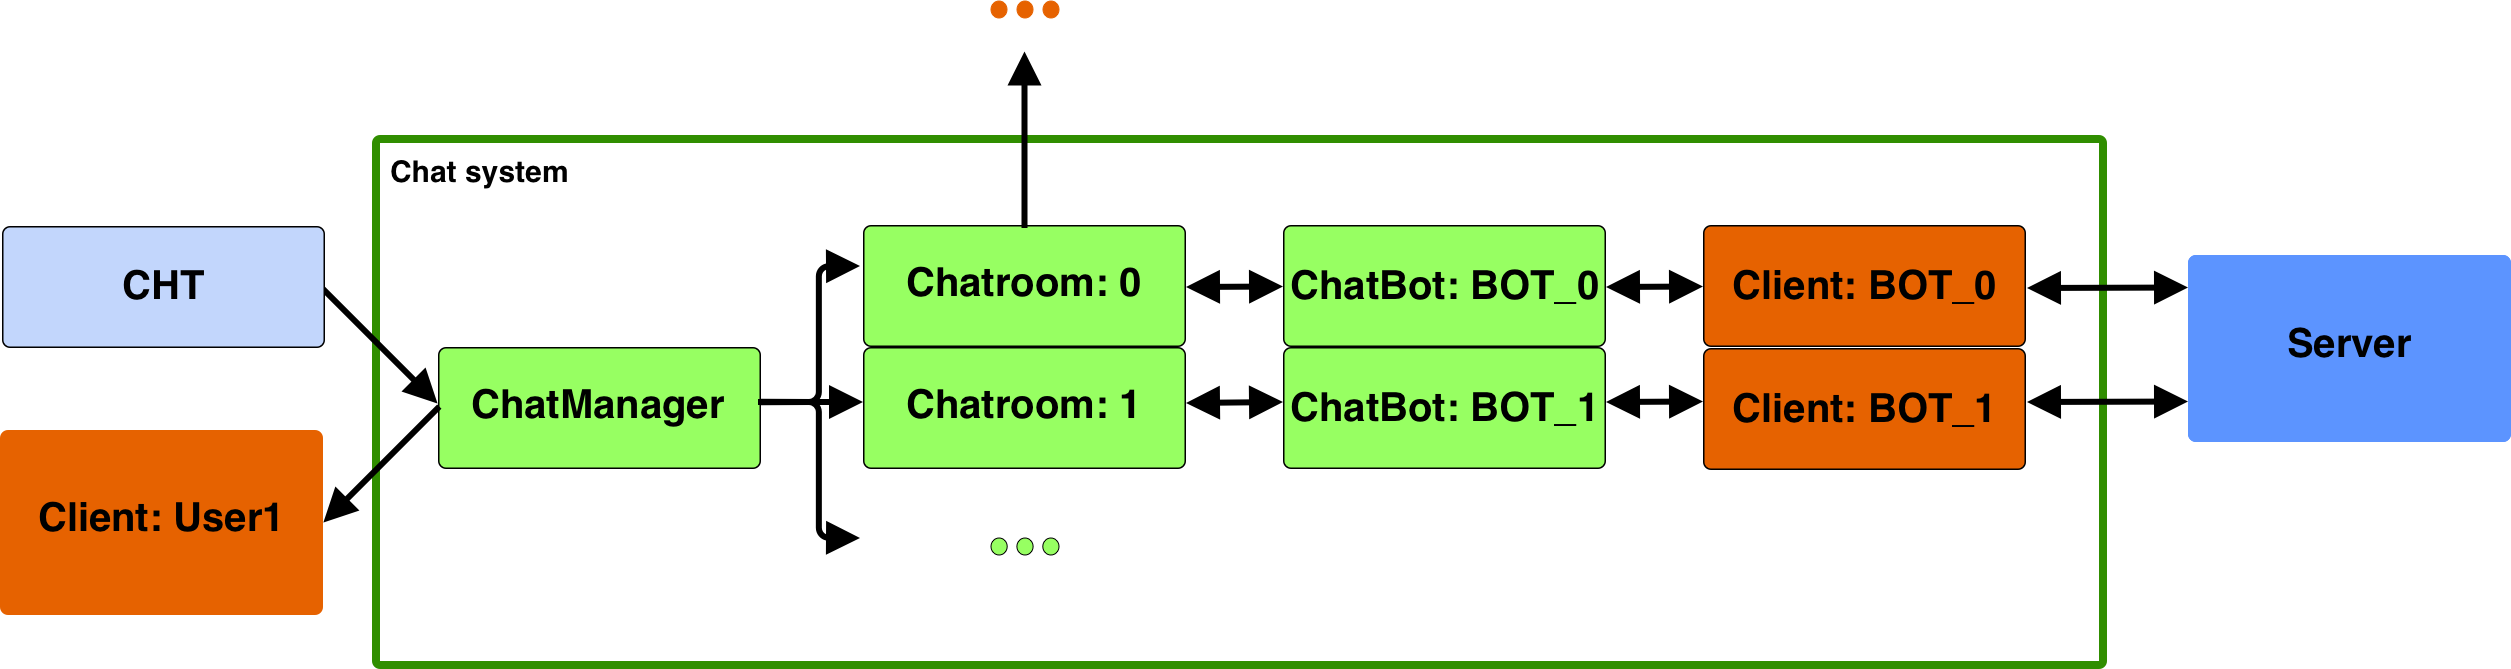
\includegraphics[width=\linewidth]{figures/chat/chat_arch.png}
	\caption{Chat system}
\end{figure}

The chat system consists of three main components as seen in the above figure\ref{fig:}:
\begin{enumerate}
	\item \textit{ChatManager}, who is in charge of providing all chat functionalities to the client, including connecting to a chatroom and sending messages.
	\item \textit{ChatRoom}, which is identified by a chatID. A Chatroom object contains a map of all connected users and their sockets, in order to be able to forward messages.
	\item \textit{ChatBot}, which is responsible to execute PUT and GET commands during a chat session. The chatbot acts exactly like a client, meaning it first has to connect to the responsible server and then send its request.

\end{enumerate}

\subsection{Database Access}
\label{sec:groupchat_chatbot}
In order to provide the chatting functionality, the server would need a socket to send to and receive messages from. However, the client also requires a socket to connect to the DB. The obvious design decision would be to add an extra socket to the client responsible for just chatting. The drawback of that idea is that the amount of TCP connections per client would get doubled, which would increase the network traffic to a large extent. In our intended use case, clients are not expected to utilize the DB heavily during chat sessions. For that reason, we could allow clients to quickly leave the chatroom to perform the DOPs and then rejoin. However, that might cause the client to miss messages while he is away, which affects the system's availability guarantee described in %TODO \ref{} server.

The approach we decided to follow in the end was creating a chatbot, whose sole purpose is executing DOPs for chat users. The chatbot acts mostly similar to a client by being able to send read and write requests to the DB. Every chatroom gets a chatbot assigned to it, which scans all incoming chat messages for DOPs, signaled by the keywords \texttt{PUT} and \texttt{GET}. Those requests are then sent to the DB and the result is returned to the chat user. In case of a read request, the \texttt{GET} operation in the message is replaced by the retrieved result. Only after this translation will the chatroom send the now modified message to every participant in the chatroom. This allows users to use stored values for communication.

\begin{figure}[h]
	\centering
	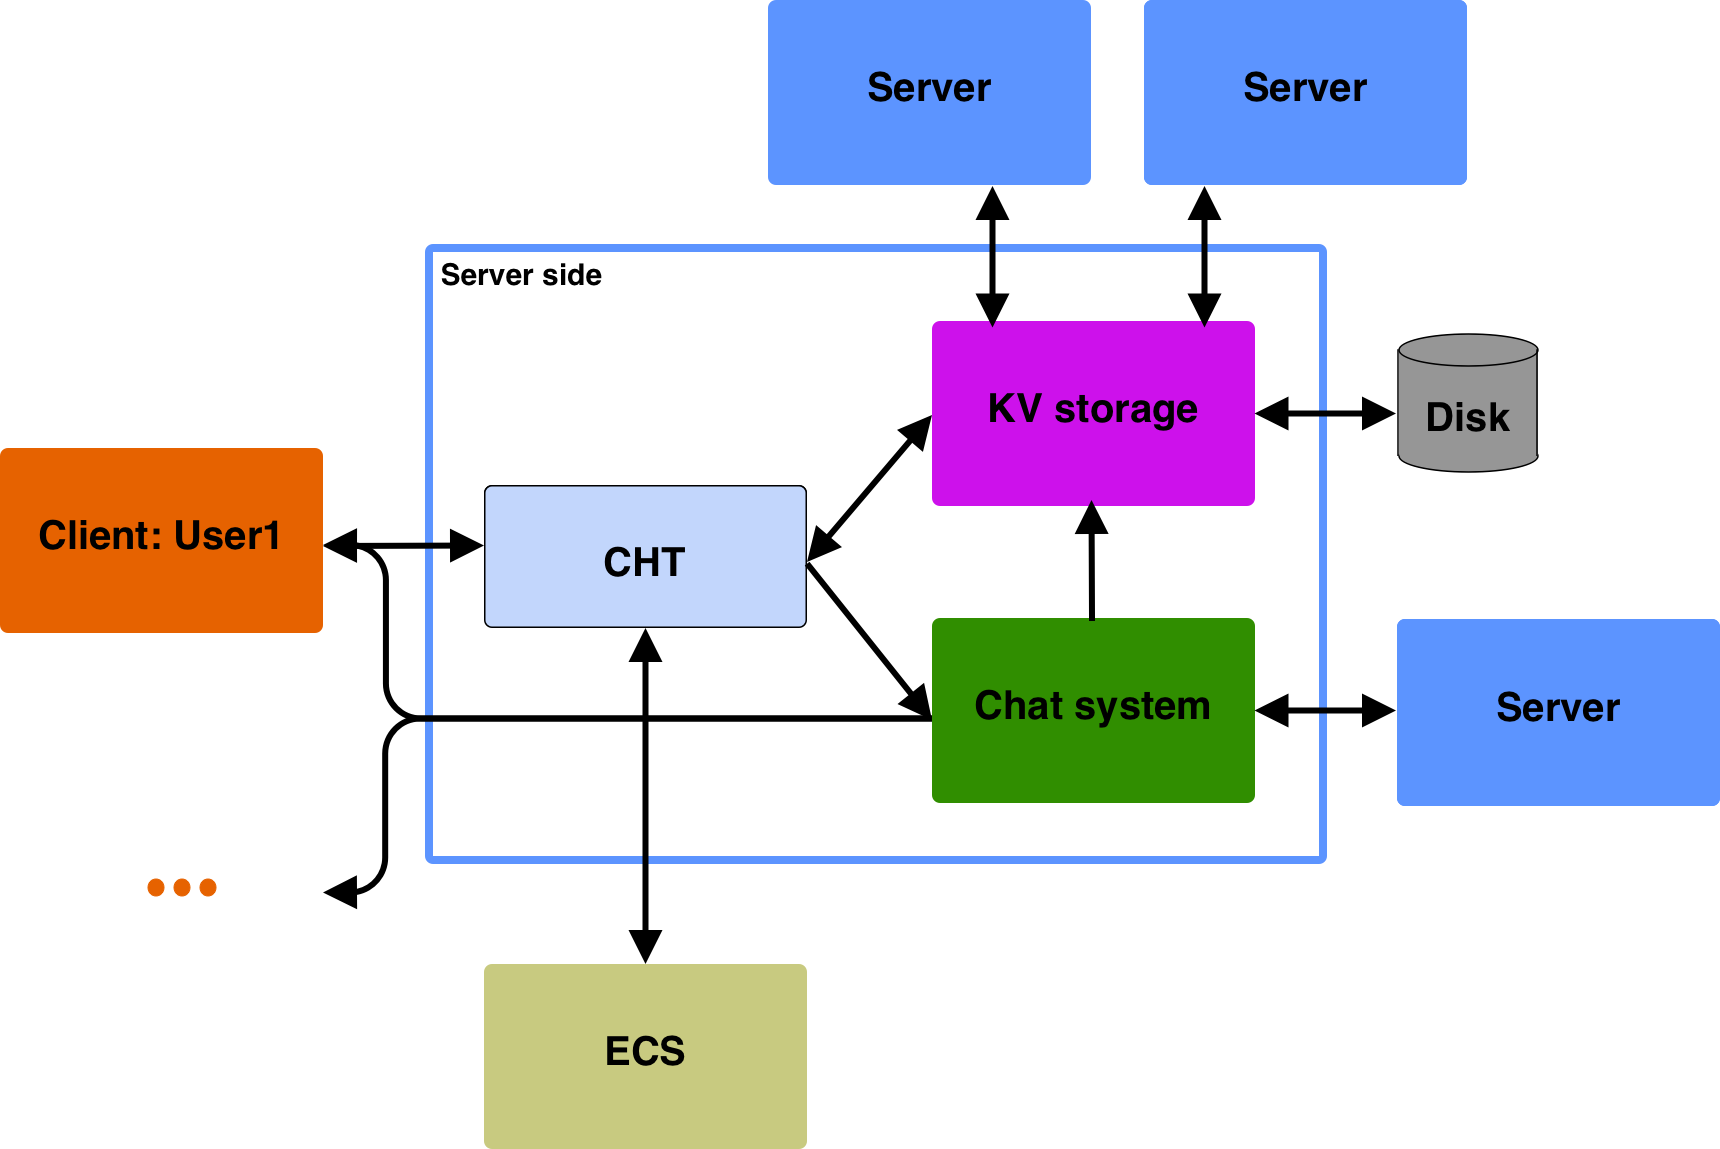
\includegraphics[width=\linewidth]{figures/chat/chat_full_arch.png}
	\caption{Server side architecture}
\end{figure}

delete??
%TODO delete?
chat system:
All chat related requests get transferred by the CHT to the ChatManager. This has a list of Chatroom objects. When a client tries to connect to a chatroom, the ChatManager checks the list whether a chatroom with the provided chatID already exists or not. In the former case, 
if the chatroom is public, the client is granted access or, in case of a private chatroom, requested to enter a password. In the event of no chatroom found with the given chatID, the client is allowed to create the chatroom by specifying its type and providing a password, if a private chatroom is chosen. In order to increase security, the password gets hashed on the client side and only the hash of the password is stored at the server side and used for validation.